\documentclass[a4paper,10pt]{article}

\usepackage{ucs}
\usepackage[utf8x]{inputenc}
\usepackage[english]{babel}
\usepackage{fontenc}
\usepackage{graphicx}
\usepackage[a4paper, top=2cm, bottom=2cm]{geometry}
\usepackage{amssymb}

\usepackage[dvips]{hyperref}
\title{String Algorithms 2013 - Assignment 3}
\author{Holger Schmeisky  201211113, Matus Tomlein 201210962}
\date{29.05.2013}

\begin{document}

\maketitle

\subsection*{State of the project}
Our algorithms work correctly and in the expected worst-case running time.

\subsection*{Insights}
For this exercise we chose python because coding in it is less verbose than in Java and we hoped to save development time. While the actual performance might be slower, because it is not a statically typed compiled language, the goal of this exercise was to measure the asymptotic runtime, so this does not matter.\\
Once again we found it useful not to stick too close to the pseudocode, but think more about what the algorithm needs to do at a certain point.
\end{itemize}

\subsection*{Problems}
During the correctness evaluation we discovered an index error in the implementation. We accessed the shift-array one position too far back, because we did not align the indices properly.

\subsection*{Evaluation of correctness}

We created a script that evaluates the results of our KMP and BA algorithm
implementations and compares them against the results of a naive algorithm
that searches for a given pattern by comparing substrings at each index
in the given string.
We used a long DNA string as an input and generated 100000 random search patterns
based on the input string.\\

According to the evaluation, both our KMP and BA implementations worked
correctly.

\subsection*{Comparison with suffix tree}

The question was:
\emph{How many times should you search for a pattern in the same text before it faster to use search from mandatory project 1 (based on constructing the suffix tree) rather than search-ba or search-kmp?}

As soon as searching for the pattern $K$ times in BA and KMP takes longer
than constructing the suffix tree for the input, we can say that searching in
the suffix tree is more efficient.
If we store the suffix tree, we have to pay the cost of creating it only once,
afterwards searching for any pattern takes just $\mathcal{O}(M)$.
However, in KMP and BA it always takes $\mathcal{O}(M+N)$ to search for a pattern.
\clearpage

\subsection*{Evaluation}
We evaluated the worst-case running time of the algorithm by generating worst-case inputs and running them repeatedly to get a running time independent of invocation overhead and computer variance. We executed the experiment on one of our laptops.\\

Worst-case inputs for both algorithms is a text consisting of just one letter, for example "AAAAAAA" and a pattern of the same letter, but with a different one at the end, e.g. "AAB". For this input the algorithms have to scan all characters of the input text once, because the pattern only mismatches on the last character of the pattern.\\

The experiment was executed on a string $A^{100}$ and patterns $A^{m}B$ with $m = 4\ldots60$ in steps of 3. We used this input, because if $n$ and $m$ are very far apart, as is the case with long texts, the expected $O(n+m)$ growth behaviour can not be observed asc clearly. We repeated each search $2000$ times, because if we search just once, we would notbe able to distinguish search time from invocation overhead and computer variance. We then measured the time searching took and plotted it. As comparison, we also plotted the graph $n+m$, scaled so that the first value matches the execution time.\\

The results in the figures below show clearly, that execution time always stays below the $n+m$ comparison line. This means that the running time grows approximately on an order of $n+m$, and because we used a worse case input, this means that the running time of our implementations of BA and KMP are no more than $\mathcal{O}(n+m)$. 

\begin{figure}[h]
  \centering
  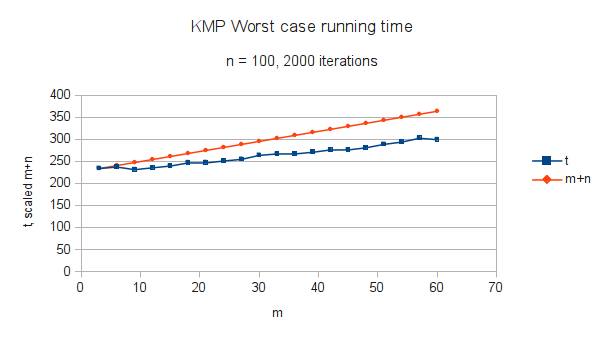
\includegraphics[scale=0.75]{./images/eval_kmp.png}
  % eval_kmp.pdf: 595x842 pixel, 72dpi, 20.99x29.70 cm, bb=0 0 595 842
  \label{fig:eval1}
\end{figure}

\begin{figure}[h]
  \centering
  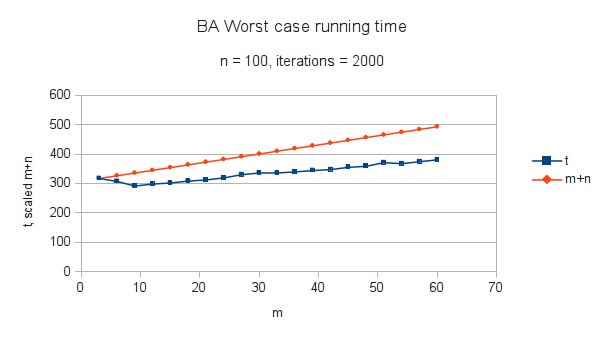
\includegraphics[scale=0.75]{./images/eval_ba - 1.png}
  % eval_kmp.pdf: 595x842 pixel, 72dpi, 20.99x29.70 cm, bb=0 0 595 842
  \label{fig:eval2}
\end{figure}



\end{document}
